% ****** Start of file aapmsamp.tex ******
%
%   This file is part of the AAPM files in the AAPM distribution for REVTeX 4-2.
%   Version 4.2a of REVTeX, January 2015
%
%   Copyright (c) 2015 American Association of Physicists in Medicine (AAPM).
%
%   See the AAPM README file for restrictions and more information.
%
% TeX'ing this file requires that you have AMS-LaTeX 2.0 installed
% as well as the rest of the prerequisites for REVTeX 4.2
%
% It also requires running BibTeX. The commands are as follows:
%
%  1)  latex  aapmsamp
%  2)  bibtex aapmsamp
%  3)  latex  aapmsamp
%  4)  latex  aapmsamp
%
% Use this file as a source of example code for your aapm document.
% Use the file aapmtemplate.tex as a template for your document.
\documentclass[%
 aapm,
 mph,%
 amsmath,amssymb,
%preprint,%
 reprint,%
%author-year,%
%author-numerical,%
]{revtex4-2}

\usepackage{graphicx}% Include figure files
\usepackage{dcolumn}% Align table columns on decimal point
\usepackage{bm}% bold math
\usepackage{xcolor}
\usepackage{hyperref}
\hypersetup{hidelinks}


\usepackage[mathlines]{lineno}% Enable numbering of text and display math

\usepackage{fancyhdr}
\pagestyle{fancy}


\makeatletter
\def\l@subsubsection#1#2{}
\makeatother



\begin{document}



\title{\includegraphics[height=1.5cm]{Images/UoE_Stacked Logo_CMYK_v1_160215.jpg} \\
Physics with Year Abroad, Literature Review:\\
Particle Identification in Modern Cherenkov Imaging Detectors}% Force line breaks with \\


\author{Daniel Markhoff}
\author{Moritz P Reiter}
\author{Jochen Schwiening}
\affiliation{School of Physics and Astronomy, University of Edinburgh, Edinburgh, UK} 
\affiliation{GSI Helmholtzzentrum für Schwerionenforschung GmbH, Darmstadt, Germany}
%update your affiliation to you correct palcement location

\date{\today}% It is always \today, today,
             %  but any date may be explicitly specified

\begin{abstract}
With major detector assemblies lining up for construction at high-energy facilities such as EIC and FAIR, 
technologies for particle identification are becoming ever more relevant. This review motivates the theory
of the field, introduces the technologies behind modern Cherenkov imaging detectors, and discusses the implementation 
of these systems into upcoming experiments. Emphasis is placed on event reconstruction techniques and the 
challenges presented by cutting-edge physics programmes. Persistent challenges include the continued development of 
photosensitive devices and deploying modern software and electronics to detector systems.
We conclude by outlining promising future developments in the field.
\end{abstract}

\maketitle

\onecolumngrid

\noindent
\textbf{Edinburgh Advisor:} Moritz P Reiter \hfill mreiter@exseed.ed.ac.uk

\noindent
\textbf{Placement Supervisor:} Jochen Schwiening \hfill j.schwiening@gsi.de

\vspace{1em}
\twocolumngrid\tableofcontents


\section{\label{sec:intro}Introduction}

% filepath: PID-in-Modern-Cherenkov/Sections/introduction.tex
% Content for the "Introduction" subsection

\label{sec:intro}

Modern high energy physics experiments rely on the performance of 
the detector systems to accurately study collision events. Cherenkov 
based detectors will play a central role in the upcoming generation of
experiments. Improving the capabilities of these detectors is the work
of thousands of physicists and engineers around the world.

This review aims to provide an introduction to the field of Cherenkov 
specific systems for particle identification (PID). We will cover the
basic principles of Cherenkov radiation, the design and operation of 
the two main types of Cherenkov detectors, and briefly over the latest 
advancements in technology.

We will begin with an overview of the necessary theoretical background
in §\ref{sec:theoretical-foundations}, and then introduce photomultipliers, 
the ever-so important devices that detect photons in §\ref{sec:photomultipliers}. Following this, we will
delve into the two/\textcolor{red}{three} main types of Cherenkov detectors in §\ref{sec:rich} and
§\ref{sec:dirc} \textcolor{red}{and §\ref{sec:neutrino-identification}}, where over the two chapters we will discuss their designs,
principles of operation, and differences. Finally, we will explore the
implementation of these detectors in upcoming experiments in §\ref{sec:applications-future-facilities},
and conclude with a discussion of some open research in §\ref{sec:current-challenges}.

\section{\label{sec:theoretical-foundations}Theoretical Foundations}

\subsection{\label{sec:cherenkov-radiation}Cherenkov Radiation}
\vspace{1em}
% filepath: /Users/danny/Documents/Courses/Year 4/Literature/Literature Review/PID-in-Modern-Cherenkov/Sections/Theoretical Foundations/cherenkov-radiation.tex
% Content for the "Cherenkov Radiation" subsection

\label{sec:cherenkov-radiation}

Cherenkov radiation is a phenomenon that occurs when a charged particle travels through a dielectric medium 
with refractive index \(n(\lambda)\) at a speed greater than the phase velocity in that medium. This effect 
was first observed by Pavel Čherenkov in 1934 \cite{Cherenkov_1937} and later explained theoretically by Ilya 
Frank and Igor Tamm \cite{Frank_1937}. 

\begin{figure}[h]
\centering
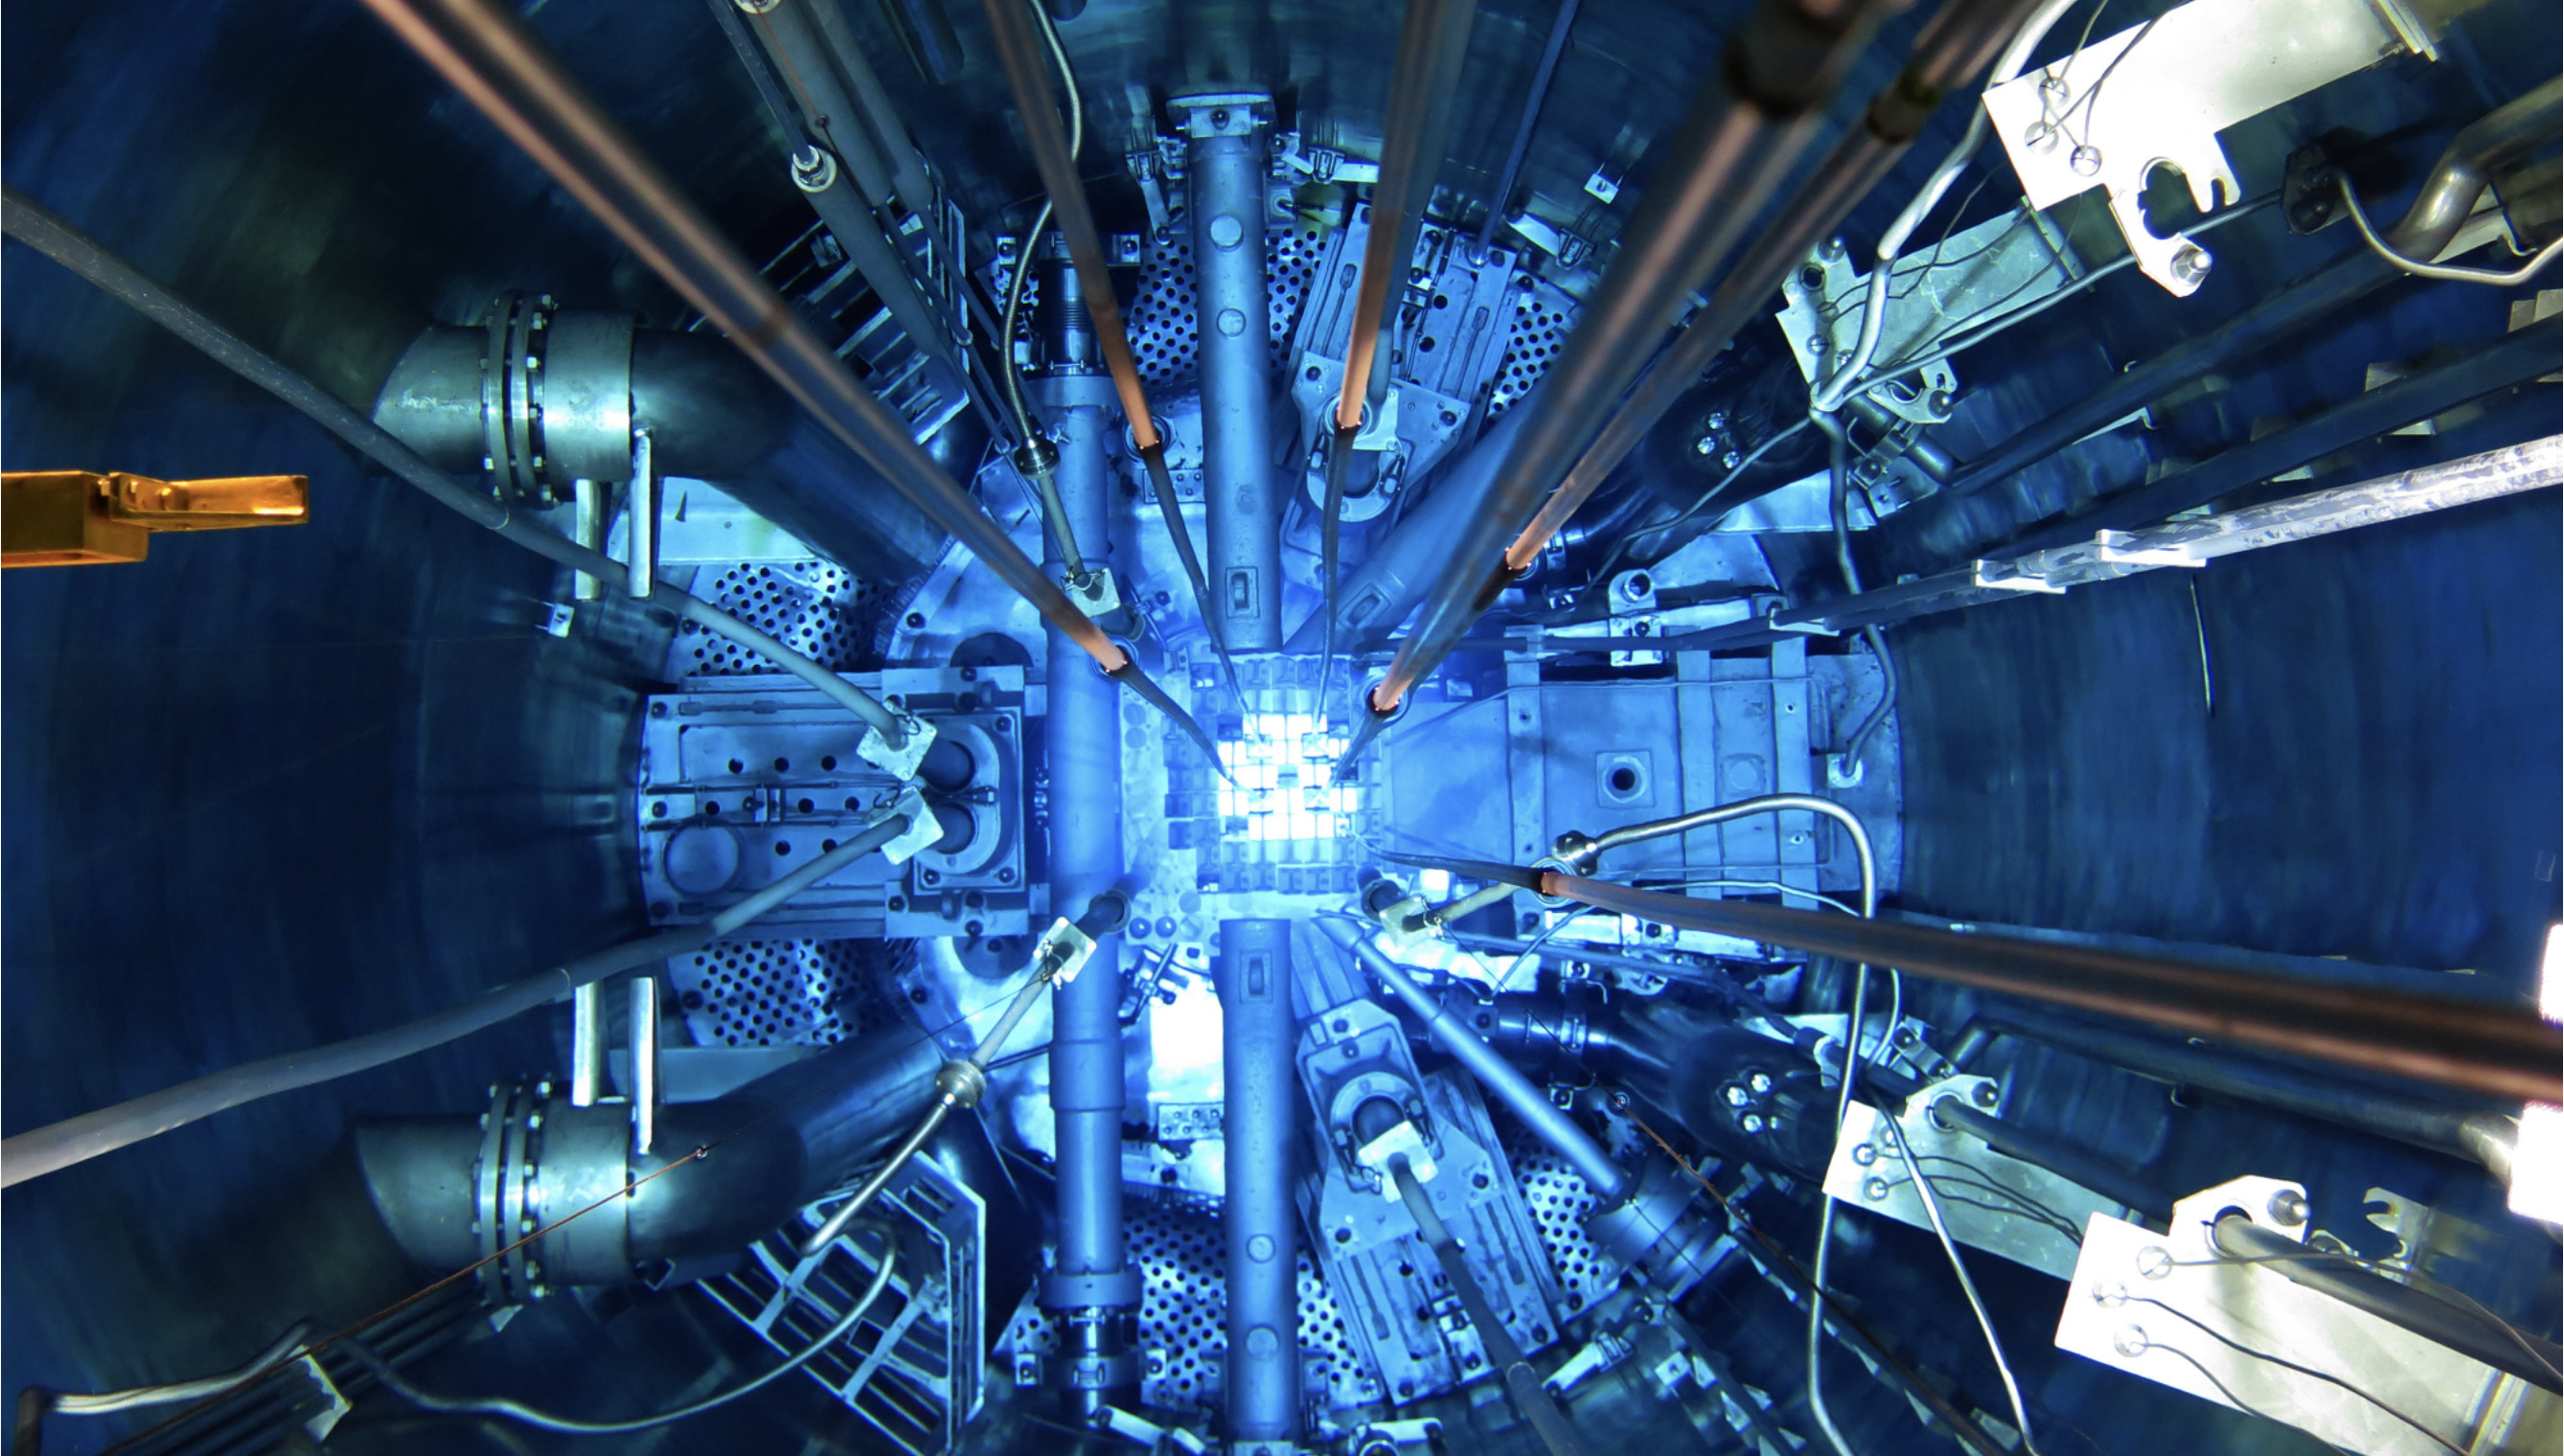
\includegraphics[width=\linewidth]{Images/cherenkov-light.png}
\caption{\textbf{Cherenkov radiation in a nuclear reactor pool.} The characteristic glow is indicative 
of relativistic electrons moving through the water. (Photo: IAEA)}\label{fig:cherenkov-light}
\end{figure}

From Maxwell's equations arises that electromagnetic propagation with wavelength \(\lambda\) will have its phase 
velocity modified by the medium it is travelling through. This leads to the idea of refractive index \(n(\lambda) = c/v\), 
defined as the ratio between the speed of light in vacuum \(c\) and the phase velocity \(v\) in the medium. The condition
for Cherenkov radiation to occur is then given by \(v > c/n\).

The Cherenkov radiation itself propagates at the phase velocity of the medium. As such, the radiation forms a 
conical wavefront with characteristic angle \(\theta\), similar to how shock cones are formed by supersonic 
aircraft. The angle \(\theta\) can be derived from simple geometric considerations shown in Fig \ref{fig:cherenkov-diagram}, yielding the following:

\begin{equation}
\cos{\theta} = \frac{v_p}{v} = \frac{c}{nv}
\label{equ:cherenkov-critical-angle}
\end{equation}

\begin{figure}[h]
\centering
\includegraphics[width=\linewidth]{Images/cherenkov-diagram.png}
\caption{\textbf{Schematic of a Cherenkov cone.} A particle travels through a medium with velocity \(v\). 
Photons are emitted at the phase velocity \(v_{p}\) and angle \(\theta\) to the path of travel of the particle, 
giving the characteristic blue shock cone.}\label{fig:cherenkov-diagram}
\end{figure}

The main principle behind a Cherenkov detector is to measure the angle \(\theta\) of the emitted photons,
which can then be used to determine the velocity \(v\) of the charged particle. With an associated momentum
measurement from a forward tracking detector, the mass of the particle can be inferred, allowing for spectroscopy.
This velocity spectroscopy for various particle species is shown in Fig \ref{fig:cherenkov-angle-COMPASS}.
It can be seen that pions, for example, will produce a larger Cherenkov angle than kaons or pions at the same momentum,
due to them being less massive.

\begin{figure}[h]
\centering
\includegraphics[width=\linewidth]{Images/cherenkov-angle.png}
\caption{\textbf{Cherenkov spectroscopy of the COMPASS RICH-1 detector at CERN.} There are clear curves for different 
particle species. These curves can be determined mathematically using \ref{equ:cherenkov-critical-angle} and relativistic
dynamics. (Photo: \cite{Tessarotto_2014})}\label{fig:cherenkov-angle-COMPASS}
\end{figure}

The energy \(dE\) emitted per unit length is given by the Frank-Tamm formula, which can be expressed as

\begin{equation}
\frac{dE}{dx} = \frac{q^2}{4\pi}\int_{v>\frac{c}{n(\omega)}}\mu(\omega)\omega\left( 1 - \frac{c^2}{v^2n^2(\omega)}\right) d\omega
\end{equation}

for a particle with charge \(q\) and frequency \(\omega\), moving through a medium with permeability \(\mu\) and 
refractive index \(n(\omega)\). The integral is taken over all frequencies where the Cherenkov condition \(v = c/n(\omega)\)
is met. By changing variables to wavelength \(\lambda\) and using that \(E = Nh\omega\), one can show that the 
number of photons \(N\) emitted per unit length is inversely proportional to the square of the wavelength. This
explains the characteristic blue of Cherenkov radiation, as shorter wavelength (blue light) photons are emitted more.




\subsection{\label{sec:relativistic-kinematics}Relativistic Kinematics}
\vspace{1em}
\input{Sections/theoretical-foundations/mass-spectroscopy.tex}
\subsection{\label{sec:optical-detector-theory}Optical and Imaging Theory}
\vspace{1em}
% filepath: PID-in-Modern-Cherenkov/Sections/theoretical-foundations/optical-detector-theory.tex
% Content for the "Optical Detector Theory" subsection

Cherenkov detectors rely heavily on the principles of optics to guide and 
detect emitted photons. Key concepts include Snell's law, total internal reflection,
and the behaviour of light in various media. Fig \nolinebreak\ref{fig:panda-bd-event-display} shows a 
simulated event display of PANDA's Barrel DIRC detector \nolinebreak\cite{Singh_2019}, illustrating how
photons are internally reflected within the radiator bars and subsequently focused going into
the trapezoidal expansion volume before being detected by the photodetector array.

\begin{figure}
\centering
\includegraphics[width=\linewidth]{Images/panda-barrel-dirc-event-display.png}
\caption{\textbf{Simulated event display of PANDA Barrel DIRC.} The blue track is a charged 
particle incident on the detector, and the yellow tracks are all Cherenkov photons. There is
a mirror at the far end of the radiator bar, causing all photons to eventually reach the
detector array.}\label{fig:panda-bd-event-display}
\end{figure}

One can imagine how important the optical properties and the geometry of the detector are
to optimise things such as photon yield and angular resolution. All things told, the PANDA 
Barrel DIRC is actually a relatively rudimentary design compared to more recent simulations
for EIC DIRC detectors, which employ more complex focusing optics to improve performance. This
will be discussed further in Sect \textcolor{red}{sec:photon-optics} and Sect \textcolor{red}{sec:applications-at-future-facilities}. 

\subsection{\label{sec:particle-physics-motivation}Particle Physics Motivation}
\vspace{1em}
% filepath: PID-in-Modern-Cherenkov/Sections/theoretical-foundations/particle-physics-motivation.tex
% Content for the "Particle Physics Motivation" subsection

\label{sec:particle-physics-motivation}

Detector assemblies are becoming ever more complex out of necessity, as the 
continual push for higher precision measurements dominates the investigation 
into quantum chromodynamics. Many types of particle physics experiments require particle identification (PID)
of hadrons such as pions, kaons and protons to observe rare processes or other heavy-ion
collisions. These PID requirements often span across extensive momentum and 
solid angle ranges; Cherenkov detectors are excellent at fulfilling these requirements.

For example, at the upcoming ePIC experiment at the Electron-Ion Collider (EIC), Cherenkov
methods will be used to provide hadron PID across essentially all high momentum ranges, as
shown in Fig \ref{fig:ePIC-pid-requirements}. These detector performance metrics will
be crucial to the experiment's physics goals towards investigating things such as nucleon 
spin, sea quarks, and high energy gluon behaviour.


\begin{figure}
\centering
\includegraphics[width=\linewidth]{Images/pid-requirements-ePIC.png}
\caption{\textbf{The ePIC PID requirements.} The pfRICH, hpDIRC and dRICH are all Cherenkov
based detectors that are expected to perform 3\(\sigma\) pion and kaon separation at momenta
between around 1 and 10 GeV\c. Here, \(\eta\) represents the pseudorapidity. (Photo: Greg Kalicy, ePIC Collaboration \cite{hpDIRC-Greg_2025})}\label{fig:ePIC-pid-requirements}
\end{figure}

To summarise, hadron detection is extremely important for flavour tagging and thus 
event reconstruction in these QCD processes. That is why Cherenkov detectors are 
imperative components of cutting edge detector assemblies.



\subsection{\label{sec:statistical-event-reconstruction-methods}Statistical and Algorithmic Foundations of Event Reconstruction}
\vspace{1em}
% filepath: PID-in-Modern-Cherenkov/Sections/theoretical-foundations/statistical-event-reconstruction-methods.tex
% Content for the "Statistical Event Reconstruction Methods" subsection

The problem of event reconstruction in modern Cherenkov detectors is to determine what happened inside the
detector based on the data obtained from the photon sensors. The most common 
current way of doing this is as a reverse ray-tracing problem. An algorithm
iterates through the possible paths a photon can take through the detector,
and evaluates a Gaussian likelihood under the hypothesis of each particle type \nolinebreak\cite{Santelj_2017}.
This likelihood is built from the spatial and temporal residuals between the
detected photon hits and the expected photon hits from the ray-tracing. For example, a Gaussian timing
likelihood can be expressed as:
\begin{equation}
    \mathcal{L}_h = \prod_{i=1}^{N} \frac{1}{\sqrt{2 \pi} \sigma} \exp \left( -{\frac{( t_i - t_{i,h}^{\text{exp}})^2}{2 \sigma^2}} \right)
\end{equation}
where \(t_i\) is the detected time of the \(i\)-th photon, \(t_{i,h}^{\text{exp}}\) is the expected time
of the \(i\)-th photon under hypothesis \(h\), and \(\sigma\) is the timing resolution of the detector system.
The hypothesis \(h\) can be for example a pion or a kaon. Note that many algorithms choose to use non-Gaussian likelihoods. 
By calculating the likelihood for each hypothesis, we can then form a log-likelihood ratio to determine which 
hypothesis is more probable:
\begin{equation}
    \Delta \log \mathcal{L} = \log \mathcal{L_{\text{kaon}} - \log \mathcal{L}_{\text{pion}}}
\end{equation}
This can be minimised across all detector hits to find the most probable particle type using various
numerical methods. Variations on this spatial method include time-imaging \nolinebreak\cite{time-imaging-roman_2020},
where the spatial information is largely ignored and instead the timing information is used to build probability density functions (PDFs)
for each particle hypothesis. The detected photon times are then compared to these PDFs to form the likelihoods. Modern algorithms
use a combination of spatial, temporal, and even angular information from other sub-detectors to build more robust likelihood functions.

In general, likelihood methods serve many detector assemblies well. However, they are in essence
a brute-force method, held back by computation limitations.
One potential new-age solution is the use of machine learning. This aims to skip 
all of the setup and calculations surrounding the likelihood methods, and rather 
let a neural network learn how the detector reacts to certain particles, implicitly encoding all of 
the likelihood-like reasoning. This has 
already seen encouraging results on Geant4 simulated data for the Hyper-Kaminokande
experiment \nolinebreak\cite{Prouse_2023} and for the PANDA Barrel DIRC \nolinebreak\cite{film-networks-markhoff_2026}.



\section{\label{sec:photomultipliers}Photon Detection Technologies}

\subsection{\label{sec:mcp-pmts}MCP-PMTs}
\vspace{1em}
% filepath: PID-in-Modern-Cherenkov/Sections/photomultipliers/mcp-pmts.tex
% Content for the "MCP-PMTs" subsection

Micro channel plate photomultipliers (MCP-PMTs) are devices that convert and 
amplify incoming photons into a measurable electrical signal. Photons incident
on a photocathode emit electrons through the photoelectric effect. These single electrons
are difficult to measure as an electrical signal, so the number of electrons
is amplified using a MCP. These are thin wafers that contain
thousands of \(\mu\)m capillaries. Via secondary emission, more electrons than 
are incident are produced \nolinebreak\cite{Bruining_1954}. This amplified electron signal is then incident on 
an anode plate, where the signal is read as an analogue voltage.

\begin{figure}[h]
\centering
\includegraphics[width=\linewidth]{Images/mcp-pmt.png}
\caption{\textbf{Cross section of a traditional MCP-PMT.} Due to the proximity of
the anode and the photocathode, we are able to determine where the incident photon 
hit. MCP-PMTs are used in an incredible range of fields, 
from blood tests, to spectroscopy, to radar jamming \nolinebreak\cite{photonics12010046}.}\label{fig:traditional-mcp-pmt}
\end{figure}

In detector physics we are interested in a few properties of MCP-PMTs. Firstly,
the quantum efficiency (QE) of the photocathode is the probability of an incident photon
producing a photoelectron; around 20\% is typical. 

Secondly, the consistency of accurate hits is of great interest. We want uniform gain
across the entire MCP-PMT, referred to as the gain behaviour. Higher gain means more distinct 
counts, and overall less uncertainty. We must also minimise faulty
signals from dark counts. Dark counts are spurious signals caused without
any incident photon, often due to thermionic emission or field emission. Balancing 
the gain behaviour, determined mostly by the anode bias, with minimising dark counts 
is a key challenge. Afterpulsing is where positive ions are created during the electron avalanche. These
positive ions accelerate backwards, towards the photocathode, causing potential damage and liberating 
secondary electrons. This creates a correlated, slightly delayed signal, appearing as a false photon hit.

Timing characteristics are also very important. The timing resolution of the MCP-PMT refers to the
uncertainty when the detector reports a single photon hit. Modern devices
are pushing 15ps time resolution \nolinebreak\cite{Lyashenko_2026}. A lower timing 
resolution allows us to be more precise with event reconstruction in detectors that rely on timing information. 
The timing resolution is also somewhat inversely correlated to the hit rate 
capability of the detector, a measure of how many incident photons the sensor can handle
before becoming too saturated.

Lastly, the lifetime of the MCP-PMT is of interest. The main factors affecting 
lifetime include overall exposure to photons, radiation damage and heat degradation. 
Minimising dark count rates and afterpulses is also crucial, as these send electrons 
to areas where they could cause chemical degradation.

MCP-PMT development is an extremely broad field spanning multiple disciplines; this overview 
just scratches the surface. The topic is central to PID and detector physics as a whole.


\subsection{\label{sec:sipms}SiPMs}
\vspace{1em}
% filepath: PID-in-Modern-Cherenkov/Sections/photomultipliers/sipms.tex
% Content for the "SiPMs" subsection
% chktex-file 
\label{sec:sipms}

Silicon photomultipliers (SiPMs) have been gaining traction recently due to 
developments in materials, leading to a great ease of manufacturing. They are
tiny compared to an MCP-PMT, due to their use of 'microcells', each containing
an avalanche photodiode (APD) and a quenching resistor, to stop the avalanche.
The review \cite{ACERBI201916} provides an excellent in depth description of SiPMs.


\begin{figure}[h]
\centering
\includegraphics[width=\linewidth]{Images/sipm.png}
\caption{\textbf{Cross section of SiPM.} SiPMs are externally biased such that 
each avalanche photodiode (APD) is at breakdown voltage, allowing for electron
avalanches. The gain from an SiPM roughly matches that of a MCP-PMT at \(10^5\) - \(10^6\). (Photo: Hamamatsu \cite{hamamatsu_2016})}\label{fig:traditional-sipm}
\end{figure}

SiPMs are much cheaper than MCP-PMTs and have a higher quantum efficiency, however suffer from a high dark count rate 
(erroneous hits) and do not have the same rate capability as MCP-PMTs. This
has led to the explosion of SiPMs in fields like positron emission photography (PET)
where precise timings are not so necessary, and where ruggedness and sturdiness
is required. SiPMs also operate at a far lower voltage than MCP-PMTs and are not affected
by magnetic fields, adding to their dependability.




\section{\label{sec:cherenkov-imaging-detectors}Cherenkov Imaging Detectors}
\vspace{1em}

\subsection{\label{sec:rich}RICH}
% filepath: PID-in-Modern-Cherenkov/Sections/rich.tex
% Content for the "Ring Imaging Cherenkov Detectors (RICH)" subsection

\label{sec:rich}

Ring Imaging Cherenkov Detectors (RICH) are a class of Cherenkov detectors that use a radiator
at a known distance from a photodetector array to measure the Cherenkov angle of incident
particles. Shown in Fig \ref{fig:simple-rich} is a simplified Geant4 simulation of a RICH
detector. 

\begin{figure}[h]
\centering
\includegraphics[width=\linewidth]{Images/simple-rich-detector.png}
\caption{\textbf{Geant4 simulation of the simplified RICH detector.} The particle track (red) 
is incident on some material with a refractive index \(n\), called the radiator. In this case,
an aerogel radiator is simulated. The resulting Cherenkov photons (gray) emitted in a 
cone are incident on a square array of sensitive photodetectors. In practice, the detector 
array is often a ring, and there are optics surrounding the device to guide photons towards 
the detector.}\label{fig:simple-rich}
\end{figure}

The Cherenkov angles are emitted in a cone around the particle track, necessitating the ring
shape; having near light speed particles directly incident on photodetectors is likely to be
expensive. The outer radius of the ring is often encased in mirrors or lenses to trap Cherenkov
photons and guide them towards the photodetector array. These optical elements are carefully manufactured
to minimise chromatic dispersion and to maintain angular resolution.

\subsection{Radiators}

Different RICH experiments use different radiator materials. Common choices include aerogel
such as in the Belle II ARICH \cite{abe2010belleiitechnicaldesign}, gaseous radiators such as in
the old LHCb RICH \cite{LHCbRICH2000technicaldesign} and (although in mostly retired detectors) 
liquids such as in the barrel CRID at SLAC \cite{barrelCRID1999SLACtechnicalreport}.

Consider the Cherenkov angle condition from Eq \ref{equ:cherenkov-critical-angle}. The radiator
refractive index \(n\) is the key parameter that determines the choice of radiator, depending on 
expected beam momenta. Higher refractive indices are necessary for lower momentum particles, which
is why we see older accelerator systems using liquid radiators with inherently higher refractive indices.

The refractive index is also wavelength dependent, which is a source of chromatic dispersion. This is an
important consideration for radiator materials, as chromatic dispersion can degrade angular resolution. The
refractive index also affects the number of Cherenkov photons produced, as per the Frank-Tamm formula in 
Eq \ref{equ:frank-tamm-formula}. There are also tricks to play with the radiator design to improve photon
yield, such as layering aerogel with different refractive indices without performance cost \cite{IIJIMA2005383}. 
Naturally though complexity comes at a cost, especially in the case of finely engineered components such as
Cherenkov radiators.

\subsection{Optics}

Optical elements are often used in RICH detectors to increase photon yield. Lenses can be used to focus Cherenkov photons
onto smaller photodetector areas, reducing cost and size. Mirrors can be used to reflect photons that would otherwise
escape the detector. Other optical tricks such as the aforementioned layered radiator (also called proxy focusing) can be
used to tighten the spread of the photon cone, allowing lower momentum charged particles to be measured. 

As an applied example, the pfRICH at the forward section of the ePIC detector makes use of conical mirrors to increase 
the acceptance angle of particle tracks which can be seen in Fig \ref{fig:pfrich-conical-mirrors}. More photons means
better angular resolution, better event reconstruction and therefore more interesting physics. That's the idea anyway.

\begin{figure}[h]
\centering
\includegraphics[width=\linewidth]{Images/pfRICH-conical-mirrors.png}
\caption{\textbf{Schematic cross section of the pfRICH.} The conical mirrors (green) near the edge of the 
vessel mean that Cherenkov photons can be detected from steeper angles than would be traditionally possible. (Photo: Brian Page, eIPC Collaboration \cite{pfRICH-Brian_2025})}\label{fig:pfrich-conical-mirrors}
\end{figure}

\subsection{Mechanics \& Integration}

Modern detectors are large, complicated systems that enjoy premium real estate. Integrating a Cherenkov detector into such an 
array presents a unique set of mechanical and design challenges. Mechanical tolerances and alignment are crucial to maintaining
accuracy. Optical elements must be precisely aligned and consistently calibrated throughout the detector lifetime, requiring
robust mechanical support and space-hungry laser calibration systems. Careful thermal and radiation management
are also necessary to ensure the longevity of photosensitive components. Consideration of the surrounding magnetic field from
the solenoid used by the TOF detectors is also necessary, especially for PMTs which are magneto-sensitive. 

Ensuring that the detector can be serviced and maintained
is also a key consideration, especially for large scale experiments that may run for decades. Some experiments are built on
rails to allow the inner detectors (RICH, TOF, trackers etc.) the be slid out for maintenance.  
These mechanical and integration challenges are often underappreciated, but are imperative to the success of a detector.


\subsection{\label{sec:dirc}DIRC}
\vspace{1em}
% filepath: PID-in-Modern-Cherenkov/Sections/dirc.tex
% Content for the "Detection of Internally Reflected Cherenkov Light" subsection

\label{sec:dirc}

There detectors, DIRC for short, are a type of Cherenkov detector that circumvent the need 
for a separate radiator by using solid transparent, typically quartz, bars to both generate and guide 
Cherenkov photons to the photodetectors. Fig \ref{fig:panda-bd-event-display} already
introduced in Section \ref{sec:optical-detector-theory} showed a Geant4 simulation of the
PANDA Barrel DIRC detector \cite{Singh_2019}, but Fig \ref{fig:panda-dirc} shows a more
detailed rendering of the barrel detector itself. 

\begin{figure}[h]
\centering
\includegraphics[width=\linewidth]{Images/panda-barrel-dirc.png}
\caption{\textbf{The PANDA Barrel DIRC.} 16 individual DIRC detectors are laid in a 
barrel-like arrangement, forming the very core of the detector array}\label{fig:panda-dirc}
\end{figure}

The basic principle of DIRC operation is similar to that of other Cherenkov detectors; charged
particles incident on a medium with refractive index \(n>1\) emit Cherenkov photons in a cone,
and we try to measure the principle angle of this cone. However, in a DIRC detector the complexity
arises from the optics of trapping and guiding the Cherenkov photons to a small array of photodetectors.
All principles from the RICH section \ref{sec:rich} apply to the DIRC also.

\subsection{Guiding Photons via Internal Reflection}
\label{sec:internal-reflection}

\subsection{Event Reconstruction}
\label{sec:event-reconstruction}

\textcolor{red}{potential conflict with §\ref{sec:statistical-event-reconstruction-methods}. Is it better to
expand that section, or to have a detailed section here with likelihood, time imaging, ML, and delete the one in the theory?}

\subsection{Timing Resolution}
\label{sec:timing-resolution}


\subsection{\label{sec:neutrino-identification}Neutrino Identification with Event Topology}
\vspace{1em}
% filepath: PID-in-Modern-Cherenkov/Sections/neutrino-identification.tex
% Content for the "Neutrino Identification with Cherenkov Detectors" subsection

\label{sec:neutrino-identification}

\subsection{Water Cherenkov Detectors}

\begin{figure}[h]
\centering
\includegraphics[width=\linewidth]{Images/super-k.jpg}
\caption{\textbf{\textcolor{red}{figure for §\ref{sec:neutrino-identification}}} (Photo: Kamioka Observatory, ICRR (Institute for Cosmic Ray Research), The University of Tokyo)}\label{fig:super-k}
\end{figure}

\subsection{Atmospheric Muons}

\begin{figure}[h]
\centering
\includegraphics[width=\linewidth]{Images/cosmic-rays.png}
\caption{\textbf{\textcolor{red}{figure for §\ref{sec:neutrino-identification}}} (Photo: Marzena Lapka, CERN)}\label{fig:cosmic-rays}
\end{figure}

\subsection{Cosmic Neutrinos}

IceCube Neutrino Observatory, use Earth as a filter to identify neutrinos from cosmic rays.

\begin{figure}[h]
\centering
\includegraphics[width=\linewidth]{Images/cosmic-neutrinos.png}
\caption{\textbf{\textcolor{red}{figure for §\ref{sec:neutrino-identification}}} (Photo: Francis Halzen \cite{iceCUBE-Halzen_2025})}\label{fig:cosmic-neutrinos}
\end{figure}

\begin{figure}[h]
\centering
\includegraphics[width=\linewidth]{Images/ice-cube-event-display.png}
\caption{\textbf{\textcolor{red}{figure for §\ref{sec:neutrino-identification}}} (Photo: Francis Halzen \cite{iceCUBE-Halzen_2025})}\label{fig:ice-cube-event-display}
\end{figure}

\section{\label{sec:applications-future-facilities}Applications at Future Facilities}

\subsection{PANDA DIRC at FAIR}
\subsection{hpDIRC at ePIC Brookhaven}
\subsection{Other Proposed Far Future Detectors}
{\color{red} might get cut}

\section{\label{sec:current-challenges}Current Challenges \& Limitations}

\vspace{1em}
% filepath: PID-in-Modern-Cherenkov/Sections/current-challenges.tex
% Content for the "Current Challenges & Limitations" subsection


banana

%\subsection{High-Rate Environments}
%\subsection{Radiation Damage}
%\subsection{Budget Constraints}


\section{Conclusion}

\hypersetup{linkbordercolor={1 1 1},citebordercolor=blue,urlbordercolor={1 1 1}}

\addcontentsline{toc}{section}{References}
\bibliographystyle{ieeetr-modified}
\bibliography{bibliography}% Produces the bibliography via BibTeX.



\end{document}
%
% ****** End of file aapmsamp.tex ******
